\section{Struktura OS – systémové jádro, monolitický systém, architektura klient-server, virtuální stroje} \label{kernel}

Operační systém si lze (opravdu zjednodušeně) představit jako program skládající se z \textit{jádra} (tj. \textit{kernel}) a \textit{systémových programů}. \textit{Systémové programy} jsou takové programy, které poskytují prostředí pro spouštění a běh \textit{aplikačních programů} (aplikace které nejsou součástí OS). Dále pak  \textit{systémová volání} fungují jako jakési API pro \textit{systémové programy} aby mohly volat funkce z jádra. (toto např. umožňuje čtení\footnote{pomocí systémového volání \textit{open}, kde můžeme nastavovat různé možnosti, jako \textit{O\_APPEND,O\_CREAT}} ze souboru nebo jejich vytváření\footnote{může se například vytvořit pomocí systémového volání \textit{open} s možností \textit{O\_CREAT}, která soubor vytvoří pokud neexistuje})

\begin{enumerate}
    \item Systémové programy -- knihovny
    \item Aplikační programy -- prohlížeč, textový editor, apod. 
\end{enumerate}
    
\begin{center}
    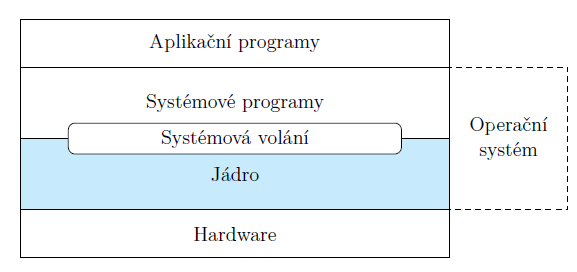
\includegraphics[scale=1]{images/OS_kernel_apps.png}
\end{center}

V Operačních Systémech zpravidla rozlišujeme dva základní režimy operací:

\begin{enumerate}
    \item režim jádra tj. privilegovaný/systémový režim
    \item uživatelský režim tj. neprivilegovaný režim
\end{enumerate}

V uživatelském režimu běží všechny aplikace, krom jádra. Více viz \ref{procesy}.

\begin{Large}
    \vspace{0,5cm} 
    \textbf{Monolitický systém}\\
\end{Large}

Jak již napovídá samotný název, \textit{monolitický systém} je systém který prakticky nemá skoro žádnou strukturu. Jádro je pouze souhrn procedur, které se navzájem volají. Tento druh jádra vzniká kompilací zdrojových kódů na objektové soubory (končící na .o), tyto objektové soubory jsou potom \textit{svázány}/\textit{spojeny} v tzv. \textit{linkeru} do jednoho spustitelného souboru. Tady vyplývá na povrch první značná nevýhoda \textit{monolitických} jader, při jakékoliv změně v jádře je třeba jej kompletně překompilovat! 

\begin{center}
    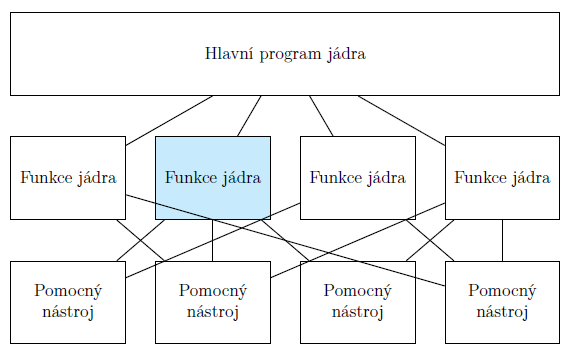
\includegraphics[scale=1]{images/OS_mono_kernel.png}
\end{center}

I když jsme si řekli, že tento systém vlastně žádnou strukturu nemá, šla by i tak popsat takto (s pomocí obrázku výše):

\begin{itemize}
    \item Hlavní program volající vyžádanou funkci
    \item Množina funkcí obsluhující systémová volání
    \item Sada nástrojů, které pomáhají funkcím
\end{itemize}

Hlavní jádro spouští funkce potřebné pro obsloužení systémových volání/přerušení (každé volání/přerušení obsluhuje jedna funkce). Pomocné nástroje pak provádí akce vyžádané funkcemi. 

\begin{large}
    \vspace{0,5cm}
    \textbf{Problémy s monolitickým jádrem a jejich řešení}\\
\end{large}

I když je monolitická architektura rychlá, má jednu značnou nevýhodu. Jedna chyba v jádře (anpř. v ovladači) může shodit celý systém. Jádro je sice od uživatelských aplikací odděleno pomocí systémových volání, a tedy chráněno před zastavením chybou v uživatelských aplikacích, ale před problémem v ovladači, jádře nebo jiných systémových službách už nikoliv.\\

Možným řešením je tzv. \textbf{modulární jádro}. Jádro jako takové obsahuje pouze části nutné pro běh, ostatní části (tzv. \textit{moduly}) jsou dynamicky načítány podle potřeby. Načítat se může při startu systému nebo i během činnosti. Výhody tohoto sytému:

\begin{itemize}
    \item Po aktualizaci/změně modulů není třeba znovu kompilovat jádro
    \item Menší velikost jádra
\end{itemize}

Moduly bývají ovladače zařízení a souborových systémů. Chyba v modulu může zastavit proces (pokud běží v procesovém kontextu v rámci obsluhy sys. volání) nebo celý systém (pokud obsluhuje sys. přerušení).

\newpage

\begin{Large}
    \vspace{0,5cm} 
    \textbf{Systém klient-server}\\
\end{Large}

Tento systém opět zmenšuje kernel až na tzv. \textit{mikrojádro}. V něm zůstanou pouze nezbytné funkce jako správa paměti, multitasking, přerušení a komunikace mezi procesy. Vše ostatní je přesunuto do tzv. \textit{serverů} což je software běžící v uživatelském režimu. Žádost o sys. volání tedy znamená, že aplikace (klient) zašle žádost \textit{serveru} kde jádro mezi nimi zprostředkovává komunikaci. \\

Z tohoto vyplývá, že chyba v \textit{serveru} nebude fatální pro celý systém. Navíc lze snadno implementovat v distribuovaných systémech (servery jsou tedy skutečné síťové servery, které vykonávají funkce jádra). Nevýhodou oproti modulárnímu jádru je v pomalejším systému. 

\vspace{0,5cm}
Lze zavést i tzv. \textbf{hybridní jádro}, kde \textit{mikrojádro} je rozšířeno o dodatečné funkce (ale ne na úrovni monolitického jádra) za účelem vyšší rychlosti. Takto např. funguje \textit{MS Windows}.

\begin{Large}
    \vspace{0,5cm} 
    \textbf{Virtuální stroje}\\
\end{Large}

Základní myšlenkou je tzv. \textit{abstrakce hardware} do několika různých prostředí, ve kterých mohou běžet oddělené operační systémy. K tomuto používáme přepínání běhu procesů na procesoru a použití konceptu virtuální paměti\footnote{Zjednodušeně, každý proces potřebuje část RAM paměti, pokud ji ovšem není dost tak se paměť procesu $"$přesune$"$ na disk do tzv. \textit{paging file}. Více: \url{https://en.wikipedia.org/wiki/Virtual_memory}}.

\vspace{0,5cm}
Každý virtuální stroj má své jádro, který musí běžet v kontextu jádra. Zároveň se však jedná o uživatelský proces, proto se vytváří virtuální uživatelský kontext a virtuální kontext jádra který však běží v uživatelském režimu na hostovacím systému. Pokud dojde ve virtuálním prostředí k sys. volání, bude obsloužení emulováno pomocí virtualizačního software (značně pomalejší než reálný systém). 


\newpage
\section{Procesy\,--\,uživatelský kontext, kontext jádra, vlákna} \label{procesy}

Začněme u toho co je to proces? Můžeme si jej představit jako program, který je realizován operačním systémem a jeden program může realizovat několik procesů. Každý proces má svůj vlastní \textit{PID} (Process IDentifier), což je celočíselná hodnota určená k identifikaci každého procesu. Tento identifikátor je přidělen procesu jádrem v okamžiku jeho vytvoření. Některé čísla jsou vyhrazena\footnote{Hodnota 0 je rezervována pro proces \textit{swapper}, který je zodpovědný za činnost virtuální paměti. Jedná se o jediný proces, který se nevytvoří voláním funkce \textit{fork} a pracuje pouze v režimu jádra. PID 1 je proces, který nelze ukončit (jelikož jej systém znovu spustí) tzv. \textit{init}, který tvoří vrchol stromové hierarchie procesů.}, ale jinak obecně neplatí, že by se podle PID dalo poznat o který proces se jedná. Identifikátor je přiřazován lineárně a při vyčerpání se začne od znovu. Lze je organizovat i do stromové struktury.

\vspace{0,5cm}
 
Procesy dělíme na \textbf{systémové} a \textbf{uživatelské}. Systémové realizují systémové programy a program jádra. Uživatelské procesy realizují ostatní uživatelské programy.  Informace o procesech se ukládají ve dvou kontextech\footnote{\textbf{Přepnutí kontextu} je něco jiného! Plánovač vybere k vykonání jiný proces, jádro pak dále udržuje ve svém kontextu stav původního procesu, aby se k němu šlo vrátit.}:

\begin{itemize}
    \item uživatelský kontext - zde se ukládají informace, které proces potřebuje pro vlastní činnost (např. programový kód)
    \item kontext jádra -  zde jsou obsaženy informace, které OS potřebuje pro správu (např. aktuální hodnota programového čítače)
\end{itemize}

\begin{Large}
    \vspace{0,5cm}
    \textbf{Uživatelský kontext}
\end{Large}

Uživatelský kontext procesu se skládá z neměnné (statické) části a dynamické části (viz Obrázky níže).

\begin{itemize}
    \item textová část (text segment) - Obsahuje programové instrukce a přístup k této části je pouze pro čtení. Díky tomu může více procesů téhož programu sdílet stejnou textovou část.
    \item datová část (data segment) - Obsahuje data, která proces potřebuje již od svého startu, tedy globální proměnné, textové řetězce, datová pole atd. 
    \item halda (heap) - Stromová struktura, kde se mohou dynamicky alokovat data za běhu programu.
    \item zásobník (stack) - Také dynamicky alokovaný, ale zde se ukládají parametry procesem volaných funkcí. Je obvyklé, že zásobník roste směrem k nižším adresám (tj. vrchol jde dolů). Jedná se o LIFO (Last-in First-out) zásobník.\footnote{Mezera mezi haldou a zásobníkem představuje volné místo, které dovoluje dynamickou změnu zásobníku a haldy během procesu.} 
\end{itemize}

\begin{figure}[H]
  \centering
  \begin{minipage}[b]{0.4\textwidth}
    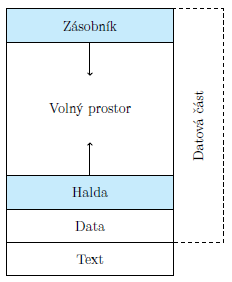
\includegraphics[width=\textwidth]{images/proc_user_context.png}
    \caption{Uživatelský kontext procesu}
  \end{minipage}
  \hfill
  \begin{minipage}[b]{0.4\textwidth}
    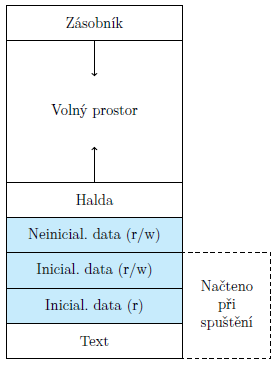
\includegraphics[width=\textwidth]{images/proc_data_segment.png}
    \caption{Datová část paměti procesu}
  \end{minipage}
\end{figure}

Datový segment lze rozdělit:

\begin{itemize}
    \item  Inicializovaná data dostupná pouze pro čtení – datové prvky inicializované programem,
    které nelze měnit.
    \item Inicializovaná data dostupná pro čtení i zápis – datové prvky inicializované programem,
    ovšem jejich hodnoty mohou být za běhu procesu měněny.
    \item Neinicializovaná data – datové prvky, které program neinicializoval. Neinicializovaná
    data lze měnit za běhu procesu.
\end{itemize}

\begin{Large}
    \vspace{0,5cm}
    \textbf{Kontext jádra}
\end{Large}

Informace potřebné pro správu procesů se mohou nacházet v \textit{řídící tabulce procesů - PCB (Process Control Block)}. V této tabulce jsou obsaženy informace o všech procesech, které jsou spuštěny. PID identifikátor navíc funguje v tabulce jako index procesu. 

\vspace{0,5cm}

V tomto kontextu jsou udržovány informaci o rozložení uživatelského kontextu, dále udržuje informace o jeho správě:
\begin{itemize}
    \item Programový čítač - obsahuje adresu následující instrukce procesu, která bude vykonána procesorem
    \item Parametry spojené s plánováním běhu procesů - priorita procesu, čas aktivity v CPU, ukazatel na plánovací frontu atd. Tyto informace jsou použity při plánování procesů, tj. rozhodování, který proces je na řadě. 
    \item Seznam vstupů a výstupů využívané procesem - například se může jednat o seznam otevřených souborů
    
    \newpage
    
    \item Stav činnosti procesu:
    \begin{enumerate}
        \item Nový - proces je vytvářený
        \item Připravený - proces čeká na to, až mu bude přidělen procesor
        \item Vykonávaný/prováděný - instrukce jsou prováděny\footnote{V tomto stavu může být vždy jenom jeden proces! Ale více programů může být ve stavu \textit{připravený} nebo \textit{čekající}}
        \item Čekající - proces čeká na nějakou událost, jako načtení dat
        \item Ukončený - proces dokončil vykonávání instrukcí
    \end{enumerate}
\end{itemize}

Po vytvoření procesu je ve stavu \textit{připravený}. Poté co je vybrán plánovačem procesů tak je \textit{vykonáván}. Vykonávání se ukončí buď dobrovolným opuštěním procesu, nebo v případu příchozího přerušení, nebo zablokování procesu z důvodu čekání na určitou událost (například na načítající se data). Při zablokování, poté co proces již není ve stavu \textit{čekání} je opět ve stavu \textit{připravený}. A celý $"$cyklus$"$ se opakuje. Pokud proces svou práci dokončí, tak přejde do stavu \textit{ukončený} do kterého lze přejít pouze ze stavu \textit{vykonávaný}! Při změně vykonávání procesu - přepnutí kontextu - se aktuální stav běhu procesu uloží v řídící tabulce procesů, ze které se i načítá poslední stav běhu procesu.

\begin{center}
    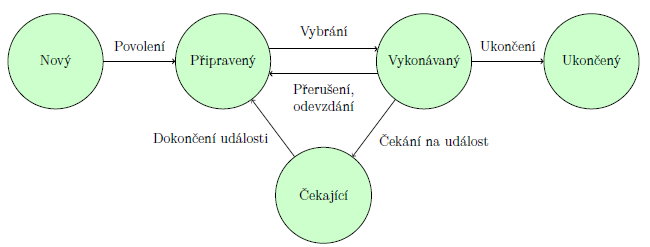
\includegraphics[scale=1]{images/proc_states.png}
\end{center}

\begin{Large}
    \vspace{0,5cm}
    \textbf{Vlákna}
\end{Large}

Lze si je představit jako stavební bloky procesů, které jsou jím vykonávané. Proces může mít jedno i více vláken, kde každé vlákno umožňuje procesu provádět pouze jeden úkol v daném čase. Je pak tedy zřejmé, že více vláken může vykonávat více různých úkolů nebo dokonce jeden stejný úkol nad různými daty (například u webového serveru). Zároveň, aby tyto úkoly šlo vykonávat ve stejném čase, musí být přítomno buď více procesorů, nebo více jader v procesoru (jedno jádro resp. jeden procesor vykonává jedno vlákno). Důležité je si zapamatovat, že každé vlákno má vlastní zásobník, ale sdílí zbytek uživatelského kontextu! (tj. datový i textový segment a haldu)

\vspace{0,5cm}

Právě skrz sdílený uživatelský kontext vláken je třeba aby programátor zajistil hladký průběh paralelizace. Například při sdílení dat mezi vlákny může dojít ke čtení nekonzistentních dat tj. k souběhu (viz \ref{sync}). 

\vspace{0,5cm}

Poté z pohledu spravování vláken je lze rozdělit na dva typy, \textit{vlákna jádra} (z programu jádra) a \textit{uživatelská vlákna} (z programů mimo jádro). Mezi uživatelskými vlákny a vlákny jádra existuje několik možných návazností/modelů:

\begin{center}
    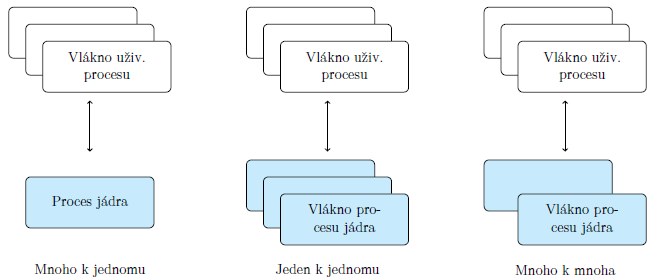
\includegraphics[scale=1]{images/thread_models.png}
\end{center}

\begin{itemize}
    \item Mnoho k jednomu - K více uživatelských vláknům přiřazuje jeden proces jádra. Použití vláken není závislé na jejich podpoře v OS a jejich správa je zajištěna často v podobě \textit{vláknových knihoven} (v uživatelském režimu). Tyto knihovny vytváří, plánují běh, přepínají a ruší vlákna. Nevýhodou je, že zavolání blokujícího sys. volání jedním z vláken zablokuje celý proces (tedy všechny vlákna), jelikož jádro nepracuje s vlákny.  
    \item Jeden k jednomu - Každé uživatelské jádro má korespondující vlákno v jádře a tedy má i na starosti jejich správu. Výhodou je, že blokující sys. volání neblokuje všechny ostatní vlákna. Dále je umožněn běh paralelně na více procesorech. Nevýhodou je značná režie, skrz vysoké množství vláken.
    \item Mnoho k mnoha - Kombinace předešlých, přiřazuje vláknům stejný nebo menší počet vláken v kernelu. Počet těchto vláken může být omezen vzhledem k aplikaci nebo druhu zařízení (např. jednoprocesorové vs. víceprocesorové)
\end{itemize}

\newpage
\section{Činnost procesů\,--\,stavy činnosti, rozšířený stavový model běhu procesů}

\newpage
\section{Plánování procesů\,--\,okamžiky rozhodnutí, plánovací algoritmy, systém priorit}

\newpage
\section{Synchronizace procesů\,--\,souběh, vzájemné vyloučení, uvíznutí procesů} \label{sync}

\newpage
\section{Správa paměti\,--\,vyměňování procesů, virtuální paměť pomocí stránkování a segmentace}

\newpage
\section{Využití paměti\,--\,přidělování paměti procesům, algoritmy přesunu stránek do odkládacího prostoru}

\newpage
\section{Souborové systémy\,--\,organizace dat na paměťovém úložišti, metody ukládání datových bloků}

\newpage
\section{Konzistence dat\,--\,data a metadata, žurnálovací souborové systémy}

\newpage
\section{Síťová část OS\,--\,stavy soketů při komunikaci, síťová systémová volání, serverové procesy}